\documentclass[a4paper,11pt]{report}
\usepackage[T1]{fontenc}
\usepackage[utf8]{inputenc}
\usepackage{lmodern}
\usepackage[spanish]{babel}
\usepackage{graphicx}
\usepackage{float} % Permite posicionar mejor las figuras y tablas
\usepackage{amsmath} % Comandos para la escritura de fórmulas matemáticas de mayor complejidad
\usepackage{amsfonts} % Proporciona fuentes matemáticas
\usepackage{amssymb} % Proporciona símbolos matemáticos de la American Mathematical Society
\usepackage{hiperref}

\title{Digit Recognizer. \\ 
  Classify handwritten digits using the famous MNIST data.\\
  Organizacion de Datos 75.06}
\author{Joaquín Blanco. Padrón 94653.\\
  Ruben Alvarado. Padrón 95686.\\
  Grupo en Kaggle: The Thompsons}

\begin{document}

\maketitle
\tableofcontents
%include == include en c
%Es preferible que cada cual tenga que trabajar en su parte
%Sin tener que lidiar con el resto. A menos que así lo quiera
\chapter{Análisis Inicial de los datos.}
Previamente al diseño de la solución, se decidió realizar un análisis de los datos de entrenamiento tal que se pueda determinar sus características y formas en que las pueden ser aprovechadas.

En principio podemos decir que contamos con 42000 imágenes de 28 píxeles de ancho por 28 píxeles de alto. Cada una esta ligada a una clase de entre 10 que pueden ser 0,1,...,9. 

En la Tabla 1.1 se puede observar el porcentaje de imágenes de cada una de las clases que existen en el set de entrenamiento y como bien se puede observar, ser puede decir que el mismo esta balanceado. 

\begin{table}[htp]
  \caption{Porcentaje de imágenes de cada una de las clases en el train}
  \label{porc}

  \begin{center}
    \begin{tabular}{|c|c|c|c|c|c|c|c|c|c|c|}
    \hline
      Clase&0&1&2&3&4&5&6&7&8&9 \\
    \hline
      Porcentaje&9.83&11.15&9.94&10.35&9.69&9.03&9.85&10.47&9.67&9.97 \\
    \hline
    \end{tabular}
  \end{center}
\end{table}

Por otro lado si realizamos un promedio de todas las imágenes y observamos los valores obtenidos, daremos cuenta de que existen pixels cuyo valor es 0. Esto nos da pie para pensar que podríamos a llegar a prescindir de algunos atributos, reduciendo así el costo computacional que requerirá procesar todos estos datos. Mas adelante en el informe veremos que esto efectivamente es así.
\begin{figure}[htp]
  \begin{center}
    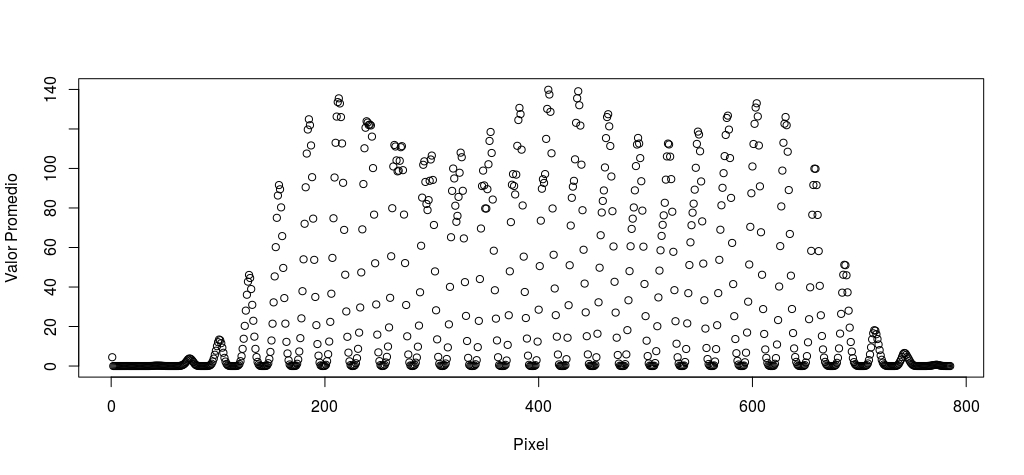
\includegraphics[width=15cm]{promImg.jpeg}
    \caption{Valores promedio de cada pixel}
    \label{promPix}
  \end{center}
\end{figure}

\chapter{Combinación de clasificadores}
La estrategia que vamos a desarrollar para cumplir con el objetivo planteado comprende llevar adelante la construcción de múltiples algoritmos de clasificación y a partir de la combinación de sus resultados lograr una mayor precisión en el reconocimiento de dígitos. En la actualidad existen múltiples estudios sobre métodos para combinar clasificadores, de entre todos ellos se decidió dar una mayor atención a aquellos que nos ofrezcan una alta precisión. Se tuvo en cuenta para la selección del tipo de combinación, los clasificadores que se van a implementar, su diversificación y su complementariedad. Cada uno de estos serán tratados mas adelante en el informe, por lo que en este capitulo nos dedicaremos exclusivamente al desarrollo de los distintos tipos de combinación que se hallaron y cual fue la elección que mejor se ajusta a nuestros objetivos e implementación.

Definiremos \textit{P} como el espacio de datos de entrada tal que $ P = C_{0}\cup...\cup C_{9} $, donde $ C_{i} $ refiere a los datos pertenecientes a la clase $ \textit{i} \in A = \{0,1,...,9\} $. Para una muestra \textit{x} extraída de \textit{P}, se puede decir que la tarea de un clasificador \textit{e} consiste en asignar un índice $ \textit{j}\in A $ a la muestra \textit{x}. Entonces \textit{e} es una función tal que $ e(x) = j  $

De acuerdo con la salida de un clasificador se definen tres tipos de problemas para los cuales se aplican distintas técnicas de combinación.
\begin{enumerate}
  \item Nivel abstracto o salida compuesta por una única clase.
  \item Nivel de rangos o listas categorizadas.
  \item Nivel de mediciones.
\end{enumerate}
Los problemas de Tipo 3 requieren que todos los clasificadores produzcan un vector de números reales de tamaño \textit{m}, siendo \textit{m} la cantidad de clases, donde en cada posición \textit{i} se guarda la probabilidad de que una muestra \textit{x} pertenezca a la clase \textit{i}. Este luego sera procesado para dotar a la muestra \textit{x} de un índice.

Por otro lado, los problemas del tipo 2 requieren que las salidas de los clasificadores sean una lista de las posibles clases a la cuales pertenezca una muestra \textit{x}. El mismo puede estar ordenada por algún criterio referente a los algoritmos que se implementaron.

Por ultimo, los problemas del tipo 1 se definen de la siguiente forma; Dados \textit{K} clasificadores individuales $ e_{k}, k = 1,...,K $ cada uno de los cuales asigna un rótulo $ j_{k} $ a una entrada \textit{x}, produciendo el evento $ e_{k}(x) = j_{k} $, se utilizan dichos eventos para construir el clasificador integrado \textit{E} que asigna $ E(x) = j $. 

Este ultimo caso admite clasificadores basados en distintas teorías y metodologías ya que solo le interesa el resultado abstracto cubriendo así todas las áreas dentro del reconocimiento de patrones. 

Es entonces que debido a su simplicidad, robustez, alta precisión en los resultados y flexibilidad que optamos por implementar métodos asociados al tipo 1. \textit{El voto por mayoría}, \textit{El voto por mayoría ponderado} o \textit{Regla de Combinación Bayesiana} son algunos de los métodos que se lograron analizar hasta el momento. De entre ellos se decidió desarrollar \textit{El voto por mayoría ponderada} dada la facilidad que comprende implementarlo\footnote{Puede que a futuro se decida cambiar esta metodología, pero por el momento se pondrá énfasis en el desarrollo de algoritmos de clasificación.}.

\section{El voto por mayoría ponderada.}
Una mejora del \textit{Voto por mayoría} consiste en considerar la confiabilidad de las respuestas de cada uno de los clasificadores individuales multiplicando cada salida por un peso. Los pesos $ w_{k} $ que expresan la competencia comparativa entre los expertos participantes, se definen como una lista de fracciones tal que
\[ \sum_{i=1}^{K}w_{i} = 1 \]
Donde \textit{K} es la cantidad de clasificadores. Cuanto mayor es la competencia de un clasificador, mayor es el valor del \textit{w} asociado.

Denotamos la desicion de un experto $ e_{k} $ que asocia una entrada \textit{x} con la clase $ i^{th} $ como $ d_{ik} $ para $ i = 0,...,9 $. La decisión que surge de la combinación de la salida de los distintos clasificadores para la clase $ i, d_{i}^{com} $, se define como:
\[ d_{i}^{com} = \sum_{k=1}^{K}w_{k} \times d_{ik} \]
La decision final $ d^{com} $ estara dada por:
\[ d^{com} = max_{i = 0,...,9} d_{i}^{com} \]

\chapter{Locality sensitive hashing (LSH)}
LSH es un conjunto de algoritmos encargados de determinar rápidamente que datos son similares entre si y representa una solución muy eficiente al problema de los vecinos mas cercanos. En este capitulo se explicara como sera su implementación en el trabajo que se esta desarrollando, algunas consideraciones a tener en cuenta y que es lo que se espera de sus resultados.

\section{LSH Euclideano}
Si consideramos cada registro del conjunto de datos de entrada como un punto de \textit{n} dimensiones\footnote{Cada punto posee inicialmente 784 dimensiones, pero posiblemente este numero se modifique a fin de reducir el costo computacional} es muy fácil pensar que KNN con distancia euclidiana es una excelente elección. Sin embargo, la búsqueda por fuerza bruta conlleva a que su aplicación sea muy poco aconsejable. 

Nuestro objetivo es pre-procesar los datos del set de train mediante una función de hashing que deposite en una mismo contenedor todos aquellos puntos que son similares a un dato \textit{x} de test y a partir de estos aplicar KNN\footnote{Se tiene en cuenta que se deberán modificar los hiper-parámetros que se utilizaron cuando solo se trataba de implementar KNN}. Siendo acordes a los conceptos de LSH, se espera que si la distancia entre \textit{x} y un punto \textit{y} del train es menor o igual a un cierto radio \textit{c}, la probabilidad de que ambos terminen en el mismo contenedor sea alta, mientras que si la distancia es mayor a \textit{c}, la probabilidad de que compartan contenedor sea muy baja. Para ello utilizaremos proyecciones aleatorias.

\section{Proyecciones aleatorias}
Para un punto \textit{x} en \textit{n} dimensiones, se puede encontrar una proyección aleatorio a $ R^{1} $ generando un vector al azar de \textit{n} dimensiones que denominaremos \textit{r} y devolviendo el producto interno entre ambos.

De acuerdo al teorema de Johnson y Lindenstrauss, una proyección aleatoria debería conservar de cierta forma la distancia entre los puntos, aunque debemos tener en cuenta que al pasar de \textit{n} dimensiones a 1, se comete un cierto error.

Para determinar en que contenedor se deben depositar cada punto solo se necesita discretizar el resultado de la proyección. Entonces, necesitamos saber el valor máximo que puede tomar el producto interno entre los puntos que se están analizando y la cantidad de contenedores que a utiliza.

Si se normalizan los datos de entrada y los vectores aleatorios son escalados en un intervalo $ [0,1] $, el resultado del producto interno sera un valor real entre $ [0,n] $, siendo \textit{n} la cantidad de dimensiones, se puede calcular el intervalo \textit{w} de la discretizacion como:
\[ w = \frac{n}{b} \]
Siendo \textit{b} la cantidad de contenedores. Finalmente definimos la función \textit{h} que para un dato \textit{x} devuelve el numero del contenedor al cual pertenece. Esta es nuestra función de hashing.
\[ h(x) = \lfloor \frac{<x,r>}{w} \rfloor  \]

Siendo coherentes con LSH, no usaremos una única función de hashing, sino mas bien $ R \times B $ funciones de hashing que estarán asociadas a $ R\times B $ tablas con una capacidad de \textit{b} contenedores.

El pre-procesamiento consiste en depositar cada uno de los puntos del train en algún contenedor en cada una de las tablas de hashing. Cada tabla esta asociado a un vector aleatorio que sera utilizado para el proceso de búsqueda. El mismo comprende tomar un dato del set de test, calcular el numero de contenedor en cada una de las para cada una de las tablas y de acuerdo a la construcción mixta que elijamos usar, obtener un conjunto de datos sobre el cual aplicar KNN. 

Supongamos que nos decidimos por una construcción del tipo AND-OR. Entonces para un dato \textit{x} se calcula el numero de contenedor para cada tabla. Se substrae de cada contenedor el conjunto de puntos que allí se depositaron y cada \textit{R} tablas realizar una intersección entre estos conjuntos. Luego finalizar con una unión de los conjuntos obtenidos.

Para este algoritmo aun no se pudo determinar los valores para \textit{R} y \textit{B}, por lo que aun esta en proceso de desarrollo. Sin embargo, es sin duda alguna uno de los clasificadores a utilizar en este trabajo.

Se espera que los resultados sean tan buenos o mejores que los obtenidos por KNN, reduciendo el tiempo que consume en el procesamiento de datos. 


\chapter{Random Forests.}
El algoritmo de Random Forests consiste en un ensamble de árboles de decisión en el que cada uno contiene un bootstrap del set de datos de entrenamiento formado por atributos elegidos de forma aleatoria. El hecho de usar un subset en lugar del set de entrenamiento completo permite evitar overfitting, y el usar subconjuntos de atributos tomados al azar ayuda a determinar cuáles son los atributos que realmente resultan más importantes para la clasificación.

Random forests fue elegido ya que ofrece una gran adaptación a casi cualquier set de datos, brindando una muy buena precisión procesando grandes cantidades de estos. Además posee un muy buen tiempo de ejecución, especialmente teniendo en cuenta su efectividad. 

Este algoritmo tiene dos hiper-parámetros: 
Por un lado la cantidad de árboles: Es fundamental para encontrar un buen funcionamiento hacer una buena elección de los mismos, ya que ante mayor cantidad de árboles, mejor clasificará el algoritmo, pero conllevará una pérdida de performance mayor. 
Por otra parte la cantidad de atributos de cada uno de los árboles:
Se eligieron en la construcción de cada árbol un conjunto al azar de atributos de nuestro set de datos, siendo dicho conjunto de una cantidad de raíz cuadrada de la cantidad total de atributos.

Se realizaron diferentes pruebas en Kaggle aplicando Random Forests al set completo de datos modificando la cantidad de árboles predictores para ver cual es la mas adecuada al problema.
Las pruebas realizadas fueron las siguientes:
\begin{enumerate}
  \item Se probó con una cantidad de 100 árboles que arrojó una efectividad de 96.514%.
  \item Se probó con una cantidad de 1000 árboles que arrojó una efectividad de 96.657%.
  \item Se probó con una cantidad de 1500 árboles que arrojó una efectividad de 96.714%.
  \item Se probó con una cantidad de 2300 árboles que arrojó una efectividad de 96.743%.
  \item Se probó con una cantidad de 3000 árboles que arrojó una efectividad de 96.771%.
\end{enumerate}
(Como antes se dijo siempre se mantuvo el segundo hiperparámetro con el valor de raiz cuadrada de la cantidad total de atributos, que es un valor recomendado para la aplicacion del algoritmo a problemas de clasificación segun la documentacion de la libreria scikit-learn de python)

Se intento correr el algoritmo con una cantidad de 10000 árboles, y luego con una de 5000 pero la performance cayó notablemente ademas que los tiempos de procesamiento se volvieron inviables.
Teniendo en cuenta que al superar la barrera de los 1000 árboles los cambios en los resultados que arrojaba el clasificador cada vez eran menos significativos pero aumentaban en gran manera el costo computacional, se tomó el tercer caso como el ideal para la aplicación de este algoritmo debido al equilibrio que brinda entre efectividad y performance.
\chapter{Conclusiones y tareas a futuro}
A lo largo del informe se explico cual sera la estrategia adoptada para la obtención de resultados mediante la combinación de múltiples algoritmos centrándonos en la simplicidad, robustez y flexibilidad. 

Para mejorar el rendimiento de la clasificación se añadirá mas datos al set de entrenamiento. En primer lugar nos proveeremos de la base de datos de CEPARMI, y en segundo, modificaremos levemente la imágenes ya dispuestas para generar nuevas imágenes. Un ejemplo de esto podría ser rotar levemente las matrices representativas de los datos mediante una matriz de rotación.

Además se están investigando nuevos algoritmos de clasificación que derivan de metodologías o teorías de la Compresión de datos.

De los algoritmos ya propuestos se espera aprender algo de los datos de entrada, tal como patrones, anomalías o métricas entre los datos. 

Se espera que agregando nuevos clasificadores y ampliando el set de entrenamiento exista una creciente mejora en el nivel de rendimiento de la aplicación.


\textbf{Bibliografía:}
\begin{enumerate}
  \item Leticia Maria Seijas, \textsc{Reconocimiento de patrones utilizando técnicas estadísticas y conexionistas aplicadas a la clasificación de dígitos manuscritos}, Universidad de Buenos Aires, Facultad de Ciencias Exactas y Naturales, 2011.
  \item Francisco Moreno Seco, \textsc{Clasificadores eficaces basados en algoritmos rápidos de búsqueda del vecino más cercano}, Universidad de Alicante, Departamento de Lenguajes y Sistemas Informáticos, 2004
  \item \textsc{LSH Euclidiano}, Universidad de Buenos Aires, Facultad de Ingeniería.
  \item Luis Argerich, \textsc{Organización de Datos, Apunte del Curso.} Universidad de Buenos Aires, Facultad de Ingeniería. 2016
  \item \textsc{Random forests, classification description} 
  \item \textsc{Que es random forest? Como funciona?}
  \item \textsc{Using Random Forests for Handwritten Digit}
  \item \textsc{Ensemble methods}
\end{enumerate}

\end{document}
